\textbf{{1. MAC地址}}

{{局域网中的每台计算机都有一个唯一的号码,}}\textbf{{称为}{MAC地址或物理地址、硬件地址。}}

每块网卡出厂即被赋予一个全球唯一的MAC地址,它被固化在网卡的ROM中,{\textbf{共48bit(6B)}},例如,01-3e-01-23-4e-3c十六进制表示,01其实是0000
0001。高24bit为厂商代码,低24bit为厂商自行分配的网卡序列号。

由于总线上使用的是广播通信,因此网卡从网络上每收到一个MAC帧,先要用硬件检查MAC帧中的MAC地址。{\textbf{如果是发往本站的帧就收下,否则丢弃}}。

\textbf{{2. MAC帧的格式}}

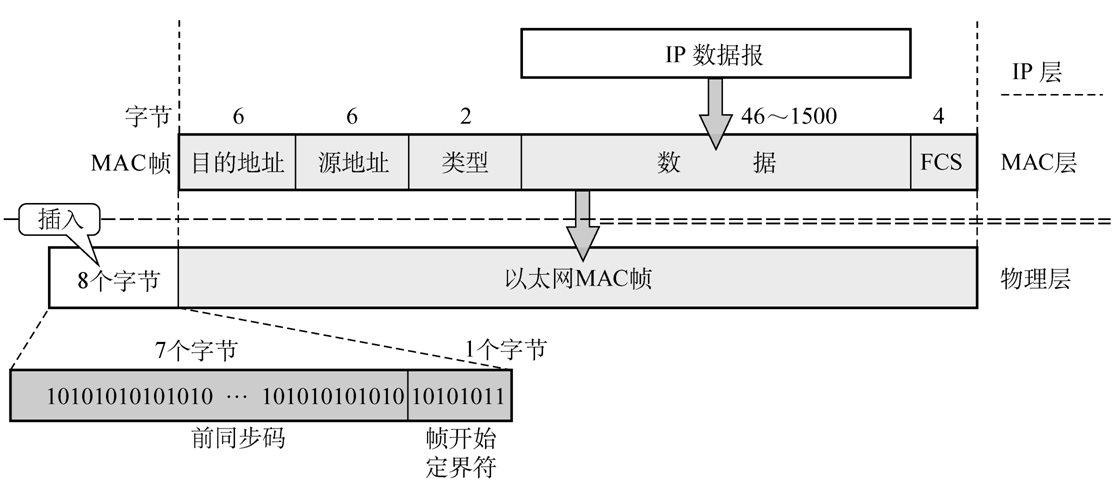
\includegraphics[width=6in]{png-jpeg-pics/651DF8353E949C3F9F8C6D9FE2187538.png}

\textbf{1.
前导码。}在帧的前面插入8B,使接收端与发送端进行时钟同步。这8B又可分为前同步码(7B)和帧开始定界符(1B)两部分。

\textbf{2. 目的地址、源地址。}均使用48bit(6B)的MAC地址。

{\textbf{3. 类型。}占2B。指出数据域中携带的数据应交给哪个协议实体处理。}

{\textbf{4.
数据。}占46~1500B。46和1500是怎么来的?首先,由CSMA/CD算法可知,以太网帧的最短帧长为64B,而MAC帧的首部和尾部的长度为18B,所以数据最短为64B-18B=
46B。其次,最大的1500B是规定的,没有为什么。}

{\textbf{5.
填充。}前面讲过,由于CSMA/CD算法的限制,最短帧长为64B,因此除去首部18B,如果数据长度小于46B,那么就得填充,使得帧长不小于64B。当数据字段长度小于46B时,需要填充至46B;当数据字段长度大于或等于46B时,则无需填充。因此,填充数据长度的范围为0~46B。}

{\textbf{6.
校验码(FCS)。}占4B。采用循环冗余码,不但需要校验MAC帧的数据部分,还要校验目的地址、源地址和类型字段,\textbf{但是不校验前导码。}}

{}
